% %
% LAYOUT_E.TEX - Short description of REFMAN.CLS
%                                       99-03-20
%
%  Updated for REFMAN.CLS (LaTeX2e)
%
\documentclass[twoside,a4paper]{refart}
\usepackage{makeidx}
\usepackage{float}
\usepackage{ifthen}
\usepackage{graphicx}
% ifthen wird vom Bild von N.Beebe gebraucht!

\def\bs{\char'134 } % backslash in \tt font.
\newcommand{\ie}{i.\,e.,}
\newcommand{\eg}{e.\,g..}
\DeclareRobustCommand\cs[1]{\texttt{\char`\\#1}}

\title{A Guide on Modelling Synapses in CellBlender and MCell}
\author{Jaron Lee}

\date{}
\emergencystretch1em  %

\makeindex 

\setcounter{tocdepth}{2}

\begin{document}

\maketitle

\begin{abstract}
    This guide aims to improve on the work by Czech et. al., by updating the guide for the MCell - CellBlender software.
\end{abstract}

%\marginlabel{Start Blender}
\newpage


%%%%%%%%%%%%%%%%%%%%%%%%%%%%%%%%%%%%%%%%%%%%%%%%%%%%%%%%%%%%%%%%%%%%
\section{Introduction}


\section{Pre- and Postsynaptic Geometry with Blender}
This section follows the paper written by Czech et. al. closely. It is expected that users will have familiarised themselves with Blender, and have read the MCell - CellBlender guide online.

\subsection{Creating a Spine Head}

\begin{enumerate}

\item   Open Blender. In the '3D View' pane, delete the default object (shortcut: x)
    
\item   Create a sphere. Select the 'UV Sphere' option from the sidebar. Below a pane called 'Add Circle' appears; set 'Segments' and 'Rings' to 16, 'Radius to '0.25'. 
        \begin{figure}[H]
        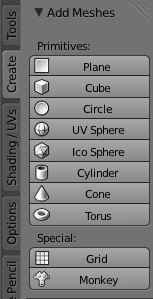
\includegraphics[scale=0.5]{spinehead1.png}
        \end{figure}

\item   Rename the sphere. Double-click the entry box below to change the default name to 'SpineHead'.
        \begin{figure}[H]
        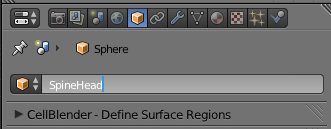
\includegraphics[scale=0.5]{spinehead2.png}
        \end{figure}

\item   Change view to see the sphere from the 'Front' view. (shortcut: 1 on numpad)

\item   Deselect the sphere (shortcut: a) and make it transparent (shortcut: z)

\item   Select the vertices to be removed. First, switch from 'Object Mode' to 'Edit Mode'. Ensure that 'Edge select' is enabled. Then use box select (shortcut: b) to capture only the faces that make up the top half of the sphere. Delete these faces (shortcut: x) and select the 'Faces' option in the delete menu.
        \begin{figure}[H]
        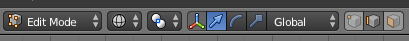
\includegraphics[scale=0.5]{spinehead3.png}
        \end{figure}

\item   Close the opening. Select the topmost vertices (remaining in 'Edge select' mode) using box select (shortcut: b). Then, extrude (shortcut: e) and click 'Edges Only' under 'Extrude' in 'Mesh Tools'.        
        \begin{figure}[H]
        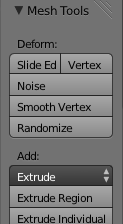
\includegraphics[scale=0.5]{spinehead4.png}
        \end{figure}
        Set the extrude distance by pressing 0 and Enter to confirm. Scale the extrusion by pressing s, 0 and Enter to confirm. Select 'Remove Doubles' under 'Mesh Tools' to remove the duplicated vertices and reconnect the triangles. Blender should note that you remove 15 vertices as a result.
        \begin{figure}[H]
        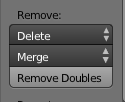
\includegraphics[scale=0.5]{spinehead5.png}
        \end{figure}
        The object should now be closed by a flat top.

\item   Subdivide triangles at the top. Unfortunately the 'Multicut tool' has been deprecated. To create set of concentric rings, first select the topmost vertices (shortcut: b). Then enter 'Knife' mode (shortcut: k), and hold down \textit{control}. This locks the knife cut to the midpoint. Click around to make a circle cut, and then press \textit{Enter} to complete the cut. Continue these cuts until the picture looks as below:
        \begin{figure}[H]
        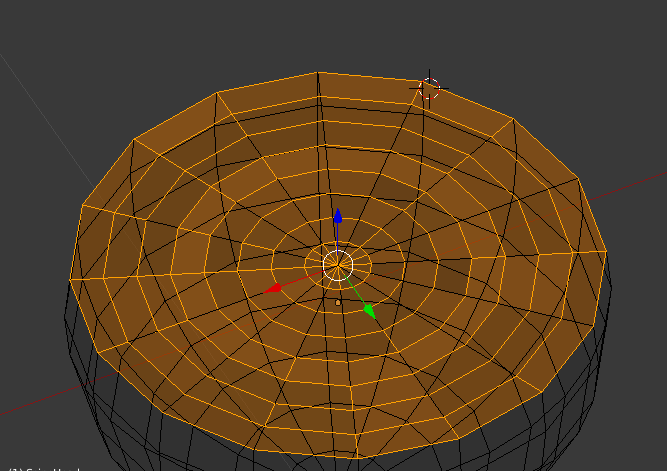
\includegraphics[scale=0.5]{spinehead6.png}
        \end{figure}
         
\end{enumerate}

\subsection{Creating a presynaptic bouton}

\begin{enumerate}
    \item   Duplicate the \textit{spine.blend} file as \textit{bouton.blend}. in \textit{bouton.blend} deselect all (shortcut: a).
    
\item   Duplicate the spine head and rotate. First, switch to 'Front' view (shortcut: 1 on numpad). Duplicate (shortcut: Shift-d, Enter) and rotate 180 degrees (shortcut: r, 180, Enter). To separate the selection of the spine heads, press p and click 'Selection'.

\item   Rename the item. Switch to 'Object Mode' (shortcut: Tab) and edit the name field to 'PresynapticBouton'.
        \begin{figure}[H]
        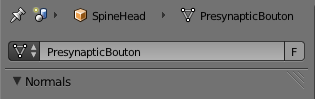
\includegraphics[scale=0.5]{bouton1.png}
        \end{figure}

\item   Shift and scale the bouton. Grab the object (shortcut: g), constrain movement to the z-axis (shortcut: z) and type 0.15, \textit{Enter} to move the object. Scale the object to be 20\% larger by typing s, 1.2, \textit{Enter}.

\item   Creating the invagination. Switch to 'Edit Mode' (shortcut: Tab) and deselect everything (shortcut: a). Select the lowermost vertices (see below) and perform the 'Select Less' operation (shortcut: Control-Minus on numpad). Click the 'Extrude Region' button under 'Add' in 'Tools', press z to constrain, and type -0.075 to extrude it upwards.
        \begin{figure}[H]
        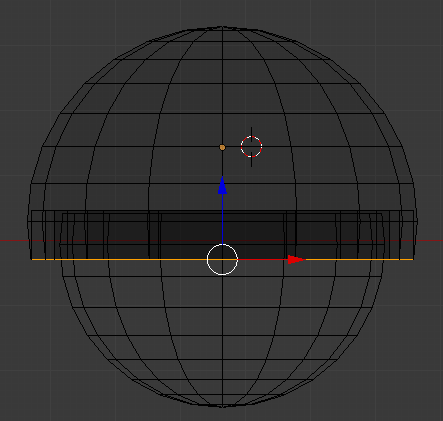
\includegraphics[scale=0.5]{bouton2.png}
        \end{figure}

\end{enumerate}

\subsection{Adding Axonal and Dendritic Extensions}

\begin{enumerate}

\item   Enter 'Edit Mode' (shortcut: Tab), and switch view to front (shortcut: 1 on numpad)

\item   Zoom in on the top of the vertex. Select the vertex by right-clicking on it, ensuring that 'Vertex mode' selection is enabled. Perform two 'Select More' operations (shortcut: Control-Plus on numpad) until two rings are highlighted. Press x, select 'Faces' on the menu, \textit{Enter} to confirm. Press b and select the vertices on the top edge using 'Box select'. Press e, click on 'Edges Only' in 'Tools' (left pane), then type z, 3.0, \textit{Enter}. This should produce an axon on the presynaptic bouton.

\item   Select the spine head. Hit \textit{Tab} to enter 'Object Mode' and right click the spine head (the bottom half-sphere) to select it. \textit{Tab} back into 'Edit Mode'

\item   Create a cylindrical spine on the spine head. As in the earlier step, select the bottom vertex, perform two 'Select More' operations, press x and select 'Faces' on the 'Erase' menu. Hit b and select the vertices that line the hole in the bottom. Press e, select 'Edges Only' in 'Tools', press z, type -2.0, \textit{Enter}. 

\end{enumerate}

\subsection{Add Synaptic Vesicles with Regions for Calcium Binding}

\begin{enumerate}
\item   Create the first vesicle. First, ensure that the object is at the origin by moving it if necessary (shortcut: g). Move the cursor to the origin (shortcut: \textit{Shift}-c). Ensure that 'Object Mode' is enabled. Under the 'Create' tab at left, select Ico-Sphere. A pane appears at lower left - change the default settings to 1 subdivision a size of 0.02. A small sphere should appear at the origin.

\item   It is necessary to rotate the vesicle. With the sphere selected, press r, x, 90, \textit{Enter} to align the sphere with the x-axis. Enter the 'Object' tab at right, and edit the name of the sphere to 'Vesicle'.

\item   Define the calcium binding region. With the vesicle still selected, change to 'Edit Mode' (shortcut: \textit{Tab}) and triangulate the faces (shortcut: \textit{Control-t}). First, select the 'Define Surface Region' tab which is under the 'Object' tab. Add a new region and name it 'vesicle\_surf' (for the surface region of the vesicle). With the vesicle selected, click 'Assign'. We must now add the vesicle to the list of mesh objects to be included in the simulation. Under the 'Scene' tab, select 'Model Objects' and add the vesicle to this list. A green tick should appear.
        \begin{figure}[H]
        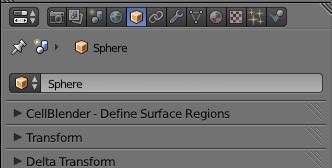
\includegraphics[scale=0.5]{vesicle1.png}
        \end{figure}

        \begin{figure}[H]
        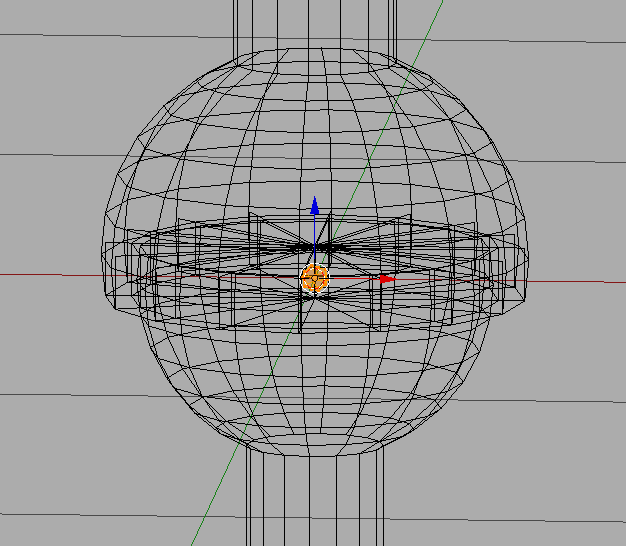
\includegraphics[scale=0.5]{vesicle2.png}
        \end{figure}

\item   Move the vesicle. Tab into 'Object Mode', press g to grab the vesicle, type x, -0.108 \textit{Enter} to move the vesicle along the x-axis. Hit g, 0.105, \textit{Enter} to move it 0.105 units along the z-axis.

\item   Duplicate the vesicle. Hit \textit{Shift}-d, g, 0.216, \textit{Enter} to move the vesicle the appropriate distance. Then, restrict visibility of the Presynaptic Bouton, select both vesicles, and under 'Define Surface Region' hit the assign button again.

        \begin{figure}[H]
        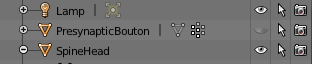
\includegraphics[scale=0.5]{vesicle3.png}
        \end{figure}


\end{enumerate}

\subsection{Defining region for voltage-gated calcium channels (VGCC)}

\begin{enumerate}
\item   Clip the existing mesh objects. Use \textit{Alt-b} to draw a box around the presynaptic terminal and the vesicles. This will only show those items and hide the rest of the model.
    
\item   Switch to overhead view. Hit 7 on the numpad to look down from above on the vesicles. We want to align the vesicles over a a few faces (note how they sit at the intersection of four faces). Select the vesicles and press r, 10 to rotate them over the appropriate faces.

\item   Select the faces. Enter 'Edit Mode' with 'PresynapticBouton' selected to observe the faces. While holding \textit{Shift} click on the faces directly under the vesicle (4 total). 

\item   Assign the selected regions. In the bottom right pane under 'Objects', go to 'Define Surface Region', and label it 'vgcc\_region'. We want this region to be an object in its own right for later selection and editing. With the region selected, press p and hit 'Selection'. Rename the object created to 'VGCC' in the top right pane. Remove the clipping box by pressing \textit{Alt-b}.
\end{enumerate}

\subsection{Defining region for postsynaptic receptors}

\begin{enumerate}
\item   Hide the presynaptic bouton and the VGCC's. Click the eye button on the top right pane for the appropriate objects.

\item   Define the postsynaptic receptor region. Right click on the postsynaptic dendrite and select the top face using the bounding box (shortcut: b). Use two 'Select Less' operations (shortcut: Control - minus on numpad) to deselect two outer rings. 

\item   Assign region. Under 'Objects' go to 'Define Surface Region' and label the receptor as 'postsynaptic\_receptor'. In CellBlender, this region will now accessed as 'SpineHead[postsynaptic\_receptor]'. Press \textit{Control - t} to triangulate the faces, and then add it under 'Scene' in 'Model Objects'.

\end{enumerate}

\section{Simulation using the CellBlender Interface}

\subsection{Adding Objects to CellBlender}
The following objects should be under 'Model Objects':

\begin{enumerate}
    \item PresynapticBouton
    \item SpineHead
    \item VGCC
    \item Vesicle
\end{enumerate}

If not, simply select the model item, triangulate (shortcut: \textit{Control}-t) and then with the item still selected add it under 'Model Objects'. This allows MCell to recognise the Blender object as part of the simulation.

\subsection{Specification of Molecules}
The following molecules will need to be added to our simulation under 'Scene' in 'Define Molecules'. The format is name of molecule, type of molecule, and diffusion constant.

\begin{enumerate}
    \item Ca, Volume, 1e-6
    \item VGCC\_C, Surface, 0
    \item VGCC\_O, Surface, 0
    \item CaBS, Surface, 0
    \item CaBS\_Ca, Surface, 0
\end{enumerate}

\subsection{Define Reactions between Molecules}
Given a set of molecules, we must define the interactions that occur when molecules meet. Under 'Define Reactions', enter the following (consists of reactants, products, and forward rate constant):

\begin{enumerate}
    \item VGCC\_C' -> VGCC\_O', 5e5
    \item VGCC\_O' -> VGCC\_C', 500
    \item VGCC\_O' -> VGCC\_O' + Ca', 1e3
    \item Ca' + CaBS' -> CaBS\_Ca', 1e7
    \item CaBS\_Ca' -> Ca' + CaBS', 500
\end{enumerate}

The apostrophes are used to indicate to CellBlender the geometry at which the reaction occurs.


\subsection{Adding Molecules to Regions}
We only want the closed VGCC's and the calcium binding sites 'CaBS' to be present when the model is initialised. All other molecules will be generated by the reactions during simulation. The following items will be added under 'Molecule Release/Placement'. 

Create a site called 'vgcc\_rel'. This will be situated on the surface named 'VGCC[vgcc\_reg]', and will represent the calcium channels. Enter the following settings.
    \begin{figure}[H]
        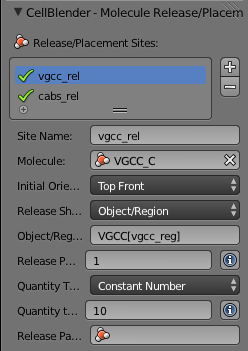
\includegraphics[scale=0.5]{settings1.png}
    \end{figure}


Similarly, create a site called 'cabs\_rel'. This will be situated on the 'Vesicle[vesicle\_surf]' and will represent the calcium release sites. Enter the following settings.
    \begin{figure}[H]
        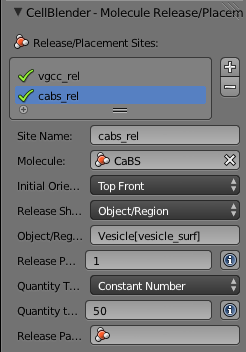
\includegraphics[scale=0.5]{settings2.png}
    \end{figure}

\subsection{Modifying Surface Classes}
It may be desirable to define surface classes so that the surfaces in the model mimic real neuron surface structures better. 

TO COMPLETE
    
\subsection{Preparing for Simulation}
A few more steps need to be copmleted before we can visualise our setup. 

First, we want to make the presynaptic bouton semi-transparent so that we can see what is occuring inside the synapse. Under the 'Material' tab (look for the little red ball) create a new material by hitting the plus sign. Click the drag-down box and change the mode from 'Object' to 'Data'. Select the presynaptic bouton, enter 'Edit Mode' and assign the new material to the selected surface. Under 'Transparency', change the alpha level to 0.3. Exit 'Edit Mode'; the surface should be semi-transparent.

    \begin{figure}[H]
        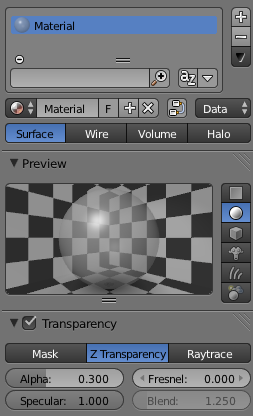
\includegraphics[scale=0.5]{settings3.png}
    \end{figure}

Then, under 'Model Initialization', set the iterations to 1000 (this is the number of frames for which the simulation will run) and the time step to 1e-6 (the amount of simulation time that passes between frames).

Under 'Reaction Output Settings', add an item for each molecule (should end up with 5 counts altogether). This setting will keep track of the number of molecules of each type currently existing in the model environment.

Finally, under 'Visualization Output Settings' click 'Export All'.

The model is now ready to go. Hit 'Run Simulation' under the 'Run Simulation' tab.
tab
\section{Troubleshooting}
\marginlabel{Simulation doesn't run} First, under 'Run Simulation' ensure that both output and error logs are being sent to file. Inspection of the error log in particular should reveal the cause of the issue. The most common error is a failure to properly assign a surface region to a Blender object - ensure that all regions are properly assigned before commencing a simulation run.

    \begin{figure}[H]
        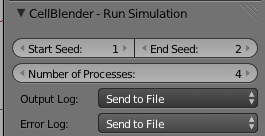
\includegraphics[scale=0.5]{trouble1.png}
    \end{figure}

\end{document}
